% QF alternative: generated from the current canonical submission-final sources.
% Author-side cache compatibility; the publisher class is unchanged.
% The class loads enumerate.sty, which is neither in its distributed ZIP nor
% in this machine's Tectonic cache. No extended enumerate syntax is used.
% Standard LaTeX list environments remain available; reject extended syntax
% in the Python builder rather than silently approximating it.
% The 2014 class also replaces kernel document/enddocument with pre-2020
% implementations. Preserve the installed kernel entry points while retaining
% all publisher typography, headings, citations and layout definitions.
\let\QFKernelDocument\document
\let\QFKernelEndDocument\enddocument
\makeatletter
\let\QFKernelOutputPage\@outputpage
\newcommand{\QFRestoreKernelDocument}{%
  \let\document\QFKernelDocument\let\enddocument\QFKernelEndDocument
  \let\@outputpage\QFKernelOutputPage}
\@namedef{ver@enumerate.sty}{2026/10/27 unused optional interface skipped}
\makeatother

\documentclass{rQUF2e}
\QFRestoreKernelDocument
% Cached Latin Modern OpenType faces; no font download or system install.
% Scalable Computer Modern-derived faces avoid absent optical-size TFM files.
\usepackage[TU]{fontenc}
\DeclareFontFamily{TU}{qflmr}{}
\DeclareFontShape{TU}{qflmr}{m}{n}{<->\UnicodeFontFile{lmroman10-regular}{\UnicodeFontTeXLigatures}}{}
\DeclareFontShape{TU}{qflmr}{m}{it}{<->\UnicodeFontFile{lmroman10-italic}{\UnicodeFontTeXLigatures}}{}
\DeclareFontShape{TU}{qflmr}{m}{sl}{<->ssub*qflmr/m/it}{}
\DeclareFontShape{TU}{qflmr}{m}{sc}{<->ssub*qflmr/m/n}{}
\DeclareFontShape{TU}{qflmr}{bx}{n}{<->\UnicodeFontFile{lmroman10-bold}{\UnicodeFontTeXLigatures}}{}
\DeclareFontShape{TU}{qflmr}{bx}{it}{<->\UnicodeFontFile{lmroman10-italic}{\UnicodeFontTeXLigatures embolden=1.8;}}{}
\DeclareFontShape{TU}{qflmr}{b}{n}{<->ssub*qflmr/bx/n}{}
\DeclareFontShape{TU}{qflmr}{b}{it}{<->ssub*qflmr/bx/it}{}
\DeclareFontFamily{TU}{qflmtt}{}
\DeclareFontShape{TU}{qflmtt}{m}{n}{<->\UnicodeFontFile{lmmono10-regular}{}}{}
\DeclareFontShape{TU}{qflmtt}{m}{it}{<->ssub*qflmtt/m/n}{}
\DeclareFontShape{TU}{qflmtt}{bx}{n}{<->ssub*qflmtt/m/n}{}
\renewcommand{\rmdefault}{qflmr}\renewcommand{\ttdefault}{qflmtt}
\normalfont

% Class declares letterpaper but predates kernel stock-size initialization.
\setlength{\paperwidth}{8.5in}\setlength{\paperheight}{11in}
% The class's 4pt footer gap collides with the restored modern output routine.
% Keep publisher typography, and explicitly fit body/header/footer to letter stock.
\typeout{QF-GEOMETRY-BEFORE textwidth=\the\textwidth; textheight=\the\textheight; footskip=\the\footskip; headheight=\the\headheight; headsep=\the\headsep; hoffset=\the\hoffset; voffset=\the\voffset; topmargin=\the\topmargin; QF-GEOMETRY-END}
\usepackage[letterpaper,hoffset=0pt,voffset=0pt,left=22mm,right=22mm,top=24mm,bottom=24mm,includeheadfoot,headheight=14pt,headsep=15pt,footskip=20pt]{geometry}
\AtBeginDocument{\typeout{QF-GEOMETRY-AFTER textwidth=\the\textwidth; textheight=\the\textheight; footskip=\the\footskip; headheight=\the\headheight; headsep=\the\headsep; hoffset=\the\hoffset; voffset=\the\voffset; topmargin=\the\topmargin; paperwidth=\the\paperwidth; paperheight=\the\paperheight; QF-GEOMETRY-END}}
% Select the required bold face before its large size; avoid loading an
% unused large regular face not present in the cache.
\renewcommand{\titlefont}{\normalfont\bfseries\fontsize{18}{22}\selectfont\centering}
\usepackage{booktabs,array,placeins}
\usepackage[unicode,breaklinks=true,hidelinks]{hyperref}
\setlength{\emergencystretch}{3em}
\setlength{\tabcolsep}{3pt}
\clubpenalty=10000\widowpenalty=10000
\newcounter{proposition}
\newcommand{\vthirteenMCSTable}{S49}
\bibpunct{(}{)}{,}{a}{}{,}
\makeatletter
\def\ps@qfsubmission{%
  \def\@oddhead{\hfil\small Quantitative Finance submission draft\hfil}%
  \let\@evenhead\@oddhead
  \def\@oddfoot{\hfil\thepage\hfil}\let\@evenfoot\@oddfoot}
\let\ps@plain\ps@qfsubmission
\makeatother
\pagestyle{qfsubmission}
\begin{document}
\title{Hard to Beat: Historical Rules versus Conditional Quantile Models for Peak Net-Position Limits}
\author{[AUTHOR NAMES TO BE COMPLETED]\\
\affil{[AFFILIATIONS TO BE COMPLETED]}}
\received{Submission draft; author details pending}
\maketitle

\begin{abstract}Dealers monitor the largest absolute position reached before a review horizon ends. We compare conditional quantile models with historical rules on hourly foreign exchange (FX) positions, weekly New York Fed positions and Commodity Futures Trading Commission (CFTC) dealer positions, matching histories and update schedules. Historical rules are hard to beat. First, FX regression lowers matched loss by 14.8\% and 16.6\% in two periods, but its ranking against a shorter rolling rule changes. Second, in the initial weekly comparisons, historical headroom beats full regression in 34 of 48 New York Fed cases; the better realized historical score wins 29 of 34 CFTC cases. Longer validation improves full regression medians in both reporting systems; CFTC short-history excess falls from 19.3\% to 4.0\%. A benchmark-default gate retains FX gains and improves weekly median performance, but leaves large individual losses. Third, lower scores need not mean lower limit costs: higher reserve charges and lower fixed breach charges generally favor regression in CFTC. Costs are illustrative, and the evidence is retrospective; the original FX evaluation period had been inspected beforehand.\end{abstract}

\begin{keywords}Peak net positions; Quantile forecasting; Historical benchmarks; Forecast comparison; Calibration; Dealer positions\end{keywords}
\begin{classcode}[TO BE COMPLETED BY AUTHOR]\end{classcode}

\section{Introduction}\label{sec:intro}

Dealer position limits concern the largest exposure reached before a review horizon ends, since an endpoint within the limit can conceal an earlier breach (Figure~\ref{fig:example}). We therefore compare historical and conditional forecasts of the sampled absolute-position peak, using the same target for every method.

Historical headroom combines the current magnitude with completed past peak behavior, while conditional models estimate additional relationships from finite historical windows. Matching histories and update schedules holds the completed-label pool and refitting clock fixed within each comparison.

\begin{figure}[htbp]\centering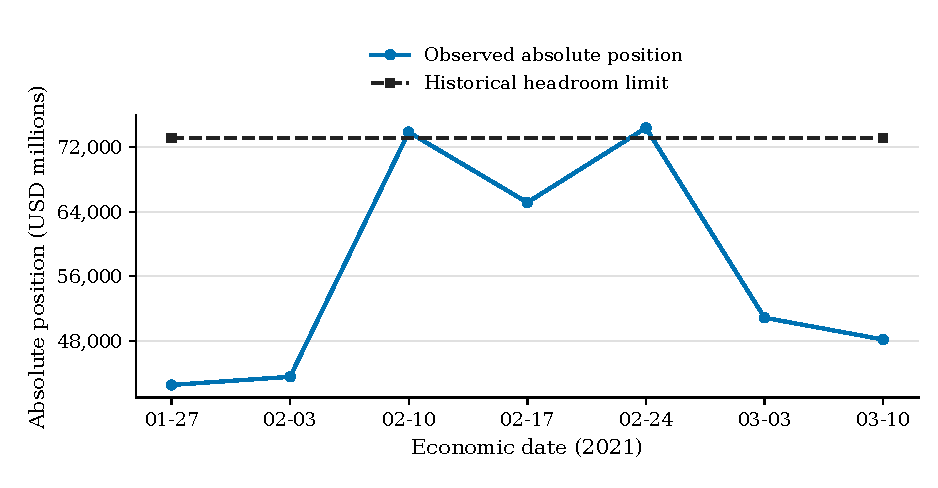
\includegraphics[width=.94\linewidth]{figures/v9-endpoint-peak-example.pdf}
\caption{A selected Treasury-bill path that returns within the reported historical limit at its endpoint after an intervening breach. The rule chooses the earliest eligible original evaluation window. Endpoint containment can conceal a peak breach.}\label{fig:example}
\end{figure}

Our evidence covers hourly foreign exchange (FX) positions, their daily aggregates, New York Fed categories and Commodity Futures Trading Commission (CFTC) dealer-category futures positions. The two official weekly reporting systems describe different aggregate exposures, so their comparisons retain separate reference procedures and source-specific scales.

Three questions organize the evaluation.

\textbf{RQ1} asks whether conditional quantile methods improve sampled peak forecasts with matched histories and update schedules.

\textbf{RQ2} asks whether those gains extend across frequencies and independently reported dealer-position aggregates.

\textbf{RQ3} asks whether score gains imply lower limit costs under reserve, breach and exceedance preferences.

The paper makes three empirical findings.

\textit{First, matched FX gains recur across periods but remain reference-dependent.} Long-history regression lowers matched loss by 14.8\% and 16.6\%, while its ranking against the shorter rolling rule changes (Section~\ref{sec:rq1}). The original-period learning curve improves with more history before surrendering part of the gain at the longest history (Figure~\ref{fig:v11-history}). Matching peak responses, completed labels and refit schedules makes these comparisons interpretable without isolating causal feature effects.

\textit{Second, longer validation improves weekly full regression medians while leaving large losses on individual tasks.} Historical controls remain competitive in both weekly reporting systems, while extended validation reduces full regression medians (Section~\ref{sec:v12-low-frequency}). The CFTC short-history median excess falls from 19.3\% to 4.0\%, and New York Fed medians also improve. A benchmark-default protocol retains FX gains and has zero weekly median excess, but 8 of 60 cases still lose by over ten percent (Section~\ref{sec:v13-rp}). These are retrospective arm-median comparisons; the horizon-six New York Fed extension also moves the validation boundary.

\textit{Third, lower scores leave limit-cost rankings sensitive to prices.} Expanded regression is cheaper in 5/34 CFTC cases at the grid center, and in 32/34 or 1/34 at opposite corners (Section~\ref{sec:cost}). Higher reserve charges and lower fixed breach charges generally favor regression, with local exceptions. These illustrative preferences motivate joint reporting of reserves, breaches and exceedance amounts, while institutional costs remain unmeasured.

Section~\ref{sec:target} defines the response. Section~\ref{sec:results} answers RQ1 and RQ2; Section~\ref{sec:cost} answers RQ3. Elementary floor and endpoint properties support the forecast definitions. The forecasting, comparison and cost-accounting procedures use standard methods.

\FloatBarrier

\section{Related literature}\label{sec:literature}

Earlier FX studies forecast signed next-hour position intervals using historical states, calendar information and local prediction methods \citep{wisniewski2020,wisniewski2024}. Their chronological training, calibration and test design reports scores and coverage together, providing a natural comparison for the present forecasting task. Our peak response instead uses a complete future path segment and the current magnitude, producing different labels and limits.


Path-risk forecasts address within-period extremes. MaxVaR studies the value at risk (VaR) of the worst cumulative portfolio return under fixed holdings and diffusion assumptions \citep{boudoukh2004}. The payment-liquidity thesis forecasts conditional maximum deficits from confidential transactions \citep{hoogen2017}. Settlement studies examine tail liquidity needs and collateral requirements \citep{petrunia2019,arjani2020}. Duffie and colleagues study dealer capacity and Treasury-market functioning, including profit and loss (PnL) quantile forecasts \citep{duffie2023}. These responses differ from the sampled absolute-position peak.


Regression quantiles target asymmetric forecast errors directly \citep{koenker1978}, while autoregressive quantiles and quantile forests supply other conditioning structures \citep{engle2004,meinshausen2006}. Consistent scores and elementary-score representations permit comparison across evaluation preferences \citep{gneiting2011,ehm2016}. Table~\ref{tab:literature} locates the present peak response, completed labels and matched historical controls.


Recent financial applications in \emph{Applied Stochastic Models in Business and Industry} study conditional quantiles and changing distributions. \citet{LeeKim2024ASMBI} develop sequential monitoring procedures for changes in conditional quantiles of heteroscedastic time series, with applications to financial return data. \citet{Pagnottoni2026ASMBI} studies distributional forecasts of high-frequency Bitcoin returns and volatility, reporting forecast errors that vary across time and quantile levels. \citet{MuddanaEtAl2025ASMBI} use quantile-regression-derived measures of tail risk and higher moments in recursive out-of-sample forecasts of gold-return volatility. The present study instead evaluates sampled position peaks against matched historical controls.

\begin{table}[htbp]\centering\footnotesize
\caption{Related studies: reported targets, data units and evaluation approaches.}\label{tab:literature}
\begin{tabular}{>{\raggedright\arraybackslash}p{2.3cm}>{\raggedright\arraybackslash}p{4.0cm}>{\raggedright\arraybackslash}p{3.9cm}>{\raggedright\arraybackslash}p{4.2cm}}\toprule
Study & Response & Data unit & Evaluation\\\midrule
\shortstack[l]{Wisniewski\\et al. (2020)} & Next-hour signed-position interval & One market maker's hourly FX positions & Pinball and interval scores; coverage tests\\
\shortstack[l]{Boudoukh\\et al. (2004)} & Worst cumulative portfolio-return quantile & Fixed portfolio under a lognormal diffusion & MaxVaR/VaR ratios; discrete-monitoring simulation\\
\shortstack[l]{van den\\Hoogen (2017)} & Conditional quantile of cumulative payment-deficit peak & ABN AMRO transaction accounts & Coverage and independence backtests\\
This study & Sampled absolute-position peak & FX positions; weekly position aggregates & Pinball loss, breaches, model confidence sets and costs\\
\bottomrule\end{tabular}
\end{table}

Matched FX gains remain reference-dependent, while longer validation reduces weekly full regression medians in two reporting systems. A benchmark-default gate still leaves large weekly losses, and illustrative cost rankings change as reserve and breach prices vary. These three findings use standard forecast tests \citep{dm1995,gw2006,mcs2011}; inventory-sensitive quoting motivates exposure monitoring \citep{avellaneda2008}. Observed position paths identify forecast behavior, leaving the effects of limits on subsequent trading decisions unmeasured.

\FloatBarrier

\section{The forecast target}\label{sec:target}

The target is the largest sampled absolute position from issue time through the stated horizon, with \(N_t\) denoting signed position and \(\mathcal F_t\) the issue-time information. The peak \(Y_{t,H}\), observed floor \(B_t\) and nonnegative headroom \(Z_{t,H}\) satisfy the following identities.


\[
Y_{t,H}=\max_{0\le h\le H}|N_{t+h}|,\qquad B_t=|N_t|,\qquad Z_{t,H}=Y_{t,H}-B_t\ge0.
\]

A feasible limit covers the current observed exposure, but Figure~\ref{fig:example} shows that endpoint containment can still conceal an earlier breach. We score reports with pinball loss and count a strict breach when the peak exceeds the limit.


\[
\rho_\tau(u)=\tau u_+ +(1-\tau)(-u)_+,\qquad I_{t,H}=\mathbf 1\{Y_{t,H}>C_{t,H}\}.
\]

\refstepcounter{proposition}\noindent\textbf{Proposition~\theproposition{} (known-floor projection).}\label{prop:floor} Suppose \(Y\ge B\) almost surely and the issue information contains \(B\). Projecting any forecast \(c\) to \(\max\{B,c\}\) weakly improves pinball loss for every outcome, with the gain shown below. The true conditional lower inverse quantile at level \(1-\alpha\) has strict exceedance probability at most \(\alpha\), including at atoms.


\[
\rho_\tau(Y-c)-\rho_\tau(Y-\max\{B,c\})=\tau(B-c)_+,\qquad \Pr(Y>q\mid\mathcal F_t)\le\alpha.
\]

\refstepcounter{proposition}\noindent\textbf{Proposition~\theproposition{} (classical endpoint-to-peak bound).}\label{prop:levy} Let future real increments be independent and individually symmetric about zero, with partial sums \(S_h\). Fix a starting position \(x\), set \(B=|x|\), and let \(q\) be the population \((1-\alpha/2)\) quantile of \(|S_H|\). The triangle inequality and the classical L\'evy maximal inequality imply the bound below. A conditional application requires these assumptions and the endpoint quantile under the law given issue-time information.


\[
\Pr\!\left(\max_{0\le h\le H}|x+S_h|>B+q\right)\le\Pr\!\left(\max_h|S_h|>q\right)\le2\Pr(|S_H|>q)\le\alpha.
\]

Supplement Sections S1--S2 retain the proofs and empirical qualifications, while Sections S3--S5 distinguish mean-reverting levels from serially correlated increments.


Separately fitted horizons can violate peak-quantile ordering, so Supplement Section S36 retains the original crossing diagnostic alongside the floor and nesting checks.


\FloatBarrier

\section{Data}\label{sec:data}

The FX application uses the hourly Net Position Time Series Dataset, reporting market-maker client-flow positions \citep{dataset,wisniewski2020}. Its 18,576 records retain source US dollar (USD) units; the later, earlier and full-prefix comparisons use distinct chronological issue grids with the same sampled-peak definition.

The weekly data are New York Fed Primary Dealer Statistics \citep{nyfeddata}. Reporting definitions follow the government-securities dealer framework and position-accounting instructions \citep{fr2004_2013,fr2004_2024}. The Treasury-bill series has 706 economic-date observations in USD millions, measuring fair-value positions aggregated as long-minus-short totals. Additional categories pass metadata and calendar checks and use complete weekly grids, with separate fits by category.

Daily aggregation takes the last recorded position on each nonempty day in the recorded calendar. It retains partial boundary days, yielding 930 days and 501 common evaluation issues, with the completed day's end serving as the issue clock. The resulting target is a peak over subsequent daily records.

The CFTC application retrospectively evaluates forecasts for a survivor universe using downloaded economic dates. It uses futures-only Dealer/Intermediary long positions minus short positions \citep{cftcTFF}. The fixed screen requires uninterrupted report weeks from 2010, stable literal codes, exchange and units. It excludes documented consolidation-code families before ranking eligible contracts by full-sample mean open interest. Seventeen contracts pass the screen, below the planned maximum of twenty. Supplement Section S30 lists every selected code and explains the eligibility rules; complete code-level exclusions remain linked there.

There are 877 weekly positions through 20 October 2026. Validation uses 52 origins; evaluation uses the last 260 eligible origins with horizon six. The evaluation position dates run from 21 September 2021 to 8 September 2026, with the final peak label completing on 20 October 2026. Refits occur every thirteen records with histories of 52 and 260, using downloaded economic dates; first-release vintages remain unobserved. Positions usually refer to Tuesday and are released Friday, so the recorded position clock differs from the public information clock.

Table~\ref{tab:v12-data} describes the aligned source records and complete six-record peaks, with monetary series expressed in USD millions. Panel summaries take nine separate medians of within-series statistics, preserving the heterogeneous exposure units across categories and contracts. Within each forecasting comparison, every method uses identical peak labels, current floors and issue origins. The same-record FX aggregation holds dealer identity fixed while changing its measurement clock and sampled response.

\begin{table}[!htbp]
\centering
\caption{Data and matched six-record peak summaries.}\label{tab:v12-data}
\begingroup\fontsize{7.5}{9}\selectfont\setlength{\tabcolsep}{2pt}
\textit{Panel A. Sources, aligned samples and existing split dates}\\[3pt]
\begin{tabular}{@{}lllllll@{}}
\toprule
Data & Frequency & Series / records & Unit & Sample & Validation & Evaluation \\
\midrule
FX, hourly & Hourly & 1 / 18,576 & USD mn & 2014-02 to 2017-01 & 2015-10 to 2015-12 & 2016-01 to 2017-01 \\
FX, daily & Day end & 1 / 930 & USD mn & 2014-02 to 2017-01 & 2015-02 to 2015-04 & 2015-05 to 2016-12 \\
Treasury bills & Weekly & 1 / 706 & USD mn & 2013-04 to 2026-10 & 2019-07 to 2020-07 & 2021-01 to 2026-04 \\
NY Fed panel & Weekly & 12 / 706 & USD mn & 2013-04 to 2026-10 & 2019-07 to 2020-07 & 2021-01 to 2026-04 \\
CFTC panel & Weekly & 17 / 877 & Contracts & 2010-01 to 2026-10 & 2020-08 to 2021-08 & 2021-09 to 2026-09 \\
\bottomrule
\end{tabular}
\par\vspace{7pt}
\textit{Panel B. Within-series mean, sample SD and empirical 95th percentile}\\[3pt]
\begin{tabular}{@{}ll*{9}{r}@{}}
\toprule
 & & \multicolumn{3}{c}{$|N|$} & \multicolumn{3}{c}{Peak $Y$} & \multicolumn{3}{c}{Headroom $Z$} \\
\cmidrule(lr){3-5}\cmidrule(lr){6-8}\cmidrule(lr){9-11}
Data & Unit & Mean & SD & 95th & Mean & SD & 95th & Mean & SD & 95th \\
\midrule
FX, hourly & USD mn & 8.92 & 10.2 & 27.6 & 11.1 & 11.7 & 30.2 & 2.15 & 5.92 & 7.96 \\
FX, daily & USD mn & 9.00 & 10.5 & 27.5 & 17.9 & 16.6 & 41.0 & 8.91 & 14.8 & 24.9 \\
Treasury bills & USD mn & 39,500 & 27,200 & 92,600 & 55,300 & 30,400 & 108,000 & 15,800 & 16,000 & 50,000 \\
NY Fed panel & USD mn & 12,400 & 8,340 & 33,300 & 16,000 & 9,040 & 37,400 & 3,750 & 3,560 & 10,500 \\
CFTC panel & Contracts & 60,200 & 46,000 & 148,000 & 81,800 & 45,600 & 169,000 & 19,900 & 20,900 & 60,600 \\
\bottomrule
\end{tabular}
\endgroup
\begin{minipage}{.98\linewidth}\footnotesize\emph{Notes.} Records are per series; complete $H=6$ peak counts are 18,570, 924, 700, 700 and 871, respectively, including the issue anchor. Earlier hourly FX validation spans 2015-04 to 2015-07 and evaluation spans 2015-07 to 2015-10; daily FX uses each nonempty source-naive day\textquotesingle s last record, and both FX periods had been inspected. SD uses $m-1$ and the empirical 95th percentile has rank $\lceil95m/100\rceil$; dollar values are in millions, panel entries are separate within-series medians without exposure pooling, and CFTC retains heterogeneous native contract counts.\end{minipage}
\end{table}


\FloatBarrier

\section{Forecasting methods}\label{sec:methods}

Unless otherwise stated, forecasts target the conditional quantile at \(\tau=19/20\). The horizons \(H\in\{6,24\}\) count subsequent source records, and each peak includes the issue position. Calendar gaps extend an FX horizon's elapsed span, while weekly and daily steps represent different review intervals under the same nineteen-to-one error-weight preference.

Historical headroom adds a corrected empirical quantile of completed headrooms to the observed magnitude:
\[
F_{t,H}=B_t+Q_j\{Z_{i,H}:i\in\mathcal T_r\},\qquad
j=\lceil(m+1)\tau\rceil,\quad m=|\mathcal T_r|.
\]
Here \(Q_j\) is the \(j\)th order statistic, and the training set contains only labels completed by refit time \(r\).
At the sensitivity level where this rank exceeds the sample size, the rank is capped at \(m\), producing the historical maximum.
This finite-sample reporting convention supplies no coverage guarantee under the observed dependence. Translated paths reanchor historical signed paths, while historical-peak quantiles are projected to the observed floor. The endpoint plug-in uses an absolute-displacement quantile; Table~\ref{tab:methods} gives the executed menus and schedules.

Ridge quantile regression links completed headroom labels to issue-known position states and calendar variables. Full regression uses 33 predictors plus an unpenalized intercept, whereas its four-feature variant uses magnitude, signed level and two root mean square (RMS) increment measures. Standardization uses only training rows with completed labels. The initial panel expansion uses five finite penalties; later decomposition and validation checks also include the intercept-only limit in this objective:
\[
(\hat a,\hat b)=\arg\min_{a,b}\left\{
\frac1m\sum_{i\in\mathcal T_r}\rho_\tau\!\left(\frac{Z_{i,H}}s-a-x_i^\top b\right)
+\frac\lambda2\|b\|_2^2\right\},\qquad
\lambda\in\{0.001,0.01,0.1,1,10,\infty\}.
\]
The intercept is unpenalized; training rows alone determine the feature transform and response scale \(s\).
Reports are \(B_t+s\max\{0,\hat a+x_t^\top\hat b\}\). The infinite-penalty candidate fixes zero slopes and chooses the lower ordinary empirical headroom quantile, also fixing the choice when intercept minimizers are nonunique.
The original menus and scale definitions remain in Table~\ref{tab:methods} and Supplement Sections S8 and S23.

Local quantiles use the k nearest historical states (KNN), with an increment-scaled variant. Filtered paths simulate positions from empirical innovations standardized by generalized autoregressive conditional heteroskedasticity (GARCH) and drawn independently with replacement \citep{hull1998,barone1999}. Quantile forests use leaf distributions; tail methods fit volatility-scaled headroom \citep{mcneilfrey2000,meinshausen2006}. Supplement Sections S7 and S11--S18 report benchmark results and failures; Section S34 links the complete legacy inventories.

Further comparisons apply delayed calibration, fixed combinations and conservative selection to the same peak response. A headroom conditional autoregressive value at risk (CAViaR) recursion and calibration wrappers follow existing methods \citep{engle2004,gibbs2021}. Calibration parameters update after outcomes mature. Fixed mean and median combinations use predefined members. Earlier conservative selection favors the strongest shrinkage whose validation loss is within one paired heteroskedasticity and autocorrelation consistent (HAC) standard error of the winner's loss. This adapts one-standard-error selection \citep{hastie2009} to paired forecast losses. The benchmark-default protocol uses a separate evidence gate against historical headroom (Section~\ref{sec:v13-rp}).

\begin{table}[htbp]\centering\small
\caption{Forecast definitions and executed menus. Codes occur here to connect with the result files. Matched histories and update schedules make the reference explicit.}\label{tab:methods}
\begin{tabular}{>{\raggedright\arraybackslash}p{2.9cm}>{\raggedright\arraybackslash}p{6.0cm}>{\raggedright\arraybackslash}p{5.3cm}}\toprule
Method & Forecast definition & Executed menu / setting\\\midrule
Historical headroom (F) & Current floor plus a quantile of completed peak headrooms & Original FX histories \{720,2880\}; weekly \{52,260\}\\
Translated path (S) & Translate completed signed paths to the current position before taking their peaks & Same completed-label pools; fixed-window and rolling-window controls\\
Historical peak (K) & Historical absolute-peak quantile projected to the current floor & Same histories and update controls\\
Quantile regression (QR) & Training-scaled headroom regression with ridge slopes and an unpenalized intercept & Original three-point menu; initial panel five-point expansion; six-point menu $\{0.001,0.01,0.1,1,10,\infty\}$\\
Local quantiles (KNN) & Neighbor headroom quantile, with a separate increment-scale variant & Training-only transforms and fixed neighbor menus; Supplement Sections S8 and S23\\
Four-feature regression (QR4) & Current signed/magnitude positions and short/long increment RMS & Original five-point menu; six-point paired comparison below\\
Endpoint plug-in (L) & Floor plus a high absolute-displacement endpoint quantile & Proposition~\ref{prop:levy}; empirical plug-in evaluated separately\\
Further benchmarks & Autoregressive replay; filtered paths; peak-tail fit; quantile forest & Existing bounded specifications; results and complete failures linked from Supplement Sections S7 and S34\\
Coverage and combinations & Delayed projected adaptive conformal inference (ACI) wrappers; symmetric absolute value (SAV) headroom recursion; fixed forecast combinations & Original-source wrapper/SAV inventory and broader combination inventory are separate\\
\bottomrule\end{tabular}
\par\smallskip\begin{minipage}{.98\linewidth}\footnotesize Training histories count completed labels. Fixed-window models refit every 24 FX records or 13 weekly records. Quantile and normalization conventions are detailed in Supplement Sections S8 and S23; this table retains the executed menus.\end{minipage}
\end{table}

\FloatBarrier

\section{Evaluation design}\label{sec:evaluation}

At refit time \(r\), only labels satisfying \(i+H\le r\) are eligible; predictors use issue-known observations and training transforms remain fixed until the next refit. Original comparisons select parameters in the preceding validation segment, while the full-prefix backcast holds its specified penalties fixed. Original weekly comparisons use 52 outer validation origins with overlapping labels.

Matched comparisons hold the completed-response history and refit schedule fixed for regression and historical headroom. The main FX reference uses a shorter rolling history, whereas the main Treasury reference shares regression's longer history and refit schedule. Tables~\ref{tab:fx} and~\ref{tab:weekly} report both alongside the other comparison sets.

Accuracy uses mean pinball loss and breaches are strict peak exceedances, scoring passive reports along the observed position paths. Paired loss differences use HAC covariance with the horizon-based bandwidth rule \citep{nw1987,dm1995}. Tables identify the small-sample adjustment and named multiplicity families \citep{holm1979,hln1997}. Hit diagnostics use a fixed spaced grid and condition the transition likelihood on its initial hit \citep{kupiec1995,christ1998}.
For paired loss differences \(d_t\), the comparison statistic and its existing bandwidth are
\[
\mathrm{DM}=\frac{\sqrt n\,\bar d}{\sqrt{\widehat\Omega_K}},\qquad
K=\min\{n-1,\max[H,\lfloor4(n/100)^{2/9}\rfloor]\},
\]
where \(\widehat\Omega_K\) is the Newey--West long-run variance estimate with Bartlett weights.


\subsection{Research design and transparency}

The original protocol fixes the two main comparisons and their reference procedures; the original FX evaluation period had already been inspected. Later analyses retain prewritten thresholds and the available local and public timing records (Supplement Sections S36, S38 and S40). Original design-object availability is reported by round. These later checks remain retrospective, and their descriptive fractions do not treat related markets as independent replications.

\subsection{Multiple-method forecast comparison}

We form a 90\% model confidence set separately for each complete source, period, horizon and history grid \citep{mcs2011}. The range statistic uses 1,000 stationary-bootstrap replications in arch 8.0.0, with block length $\max\{H,\lceil n^{1/3}\rceil\}$. All complete saved procedures enter on matching origin grids and targets, while incomplete prior methods remain explicitly unavailable. The nominal level presumes suitable loss dependence; it does not account for earlier research-stage model development.

Exact duplicate loss columns enter the bootstrap once, and their procedure labels are restored afterward. Historical reports are merged only after their full forecasts and targets match, while rolling references remain distinct. Several methods can produce identical losses, so one surviving loss pattern need not mean that only one method survives. The fractions summarize related tasks, with no independent cross-market pooled test.

\FloatBarrier

\section{Results}\label{sec:results}

\subsection{RQ1: matched accuracy and reference stability}\label{sec:rq1}

Long-history FX regression beats matched historical headroom in both periods, yet its ranking against the shorter rolling reference reverses in the earlier period (Table~\ref{tab:fx}). This distinction makes the reference procedure part of the substantive finding, since a conditioning gain alone does not determine the overall ranking.

Beyond the matched long-history case, short-history FX regression performs poorly at the longer horizon. Loss rises by 31.5\% against matched historical headroom. Regression records 924 breaches against 427 for the reference; the full horizon map retains the other adverse comparisons. This adverse case shows why the matched long-history gain cannot be generalized across horizons and training-window lengths.

Delayed calibration retains the later matched FX gain, although its breach count remains slightly higher than wrapped historical headroom on common origins (Table~\ref{tab:fx}). Calibration therefore changes breach frequency, while the distinct score and hit rankings persist on the common comparison grid.

Supplement Sections S20--S21 and S26 report the state, target-level and overlapping full-prefix comparisons (Tables S19--S21 and S25--S26).

\begin{table}[htbp]\centering\small
\caption{Long-history short-horizon FX regression under two references and periods. Negative percentages favor regression. Matched gains recur while the rolling-reference direction changes.}\label{tab:fx}
\begin{tabular}{>{\raggedright\arraybackslash}p{2.6cm}>{\raggedright\arraybackslash}p{4.4cm}>{\raggedleft\arraybackslash}p{2.5cm}>{\raggedleft\arraybackslash}p{1.5cm}>{\raggedright\arraybackslash}p{3.2cm}}\toprule
Period / procedure & Reference & Loss change (\%) & Issues & Strict breaches (regression / reference)\\\midrule
Later / original main comparison & Shorter-history rolling headroom & -12.66 & 6625 & 376 / 332\\
Later / matched & Same-history fixed-window headroom & -14.77 & 6625 & 376 / 360\\
Earlier / original structure & Shorter-history rolling headroom & +3.17 & 1440 & See complete earlier-period tables\\
Earlier / matched & Same-history fixed-window headroom & -16.62 & 1440 & 20 / 16\\
Later / coverage-wrapped & Same-history wrapped headroom & -15.00 & 6625 & 329 / 328\\
\bottomrule\end{tabular}
\par\smallskip\begin{minipage}{.98\linewidth}\footnotesize Regression uses history 2880 and horizon 6; the original rolling reference uses 720. The earlier matched comparison is the original three-penalty regression, not the later one-standard-error selection rule. The wrapper comparison is a separate finite projected delayed ACI-style exercise.\end{minipage}
\end{table}

\FloatBarrier
\subsection{How much history does FX regression need?}\label{sec:fx-history}

The fixed-period, short-horizon learning curve shows that more history helps only over part of the tested range (Figure~\ref{fig:v11-history}). Full regression moves from higher loss at the shortest history to its largest matched gain at an intermediate history. The gain is smaller at the longest history, while the four-feature curve changes sign within the tested range. Both curves use the original FX period and their original penalty menus; regression is compared with its own matched historical reference at each history length. Supplement Section S35 retains the full contrasts and synthetic confirmation summary. Within the tested configurations, the history and menu comparisons link conditional gains to history length and the availability of strong shrinkage.

\begin{figure}[!htbp]\centering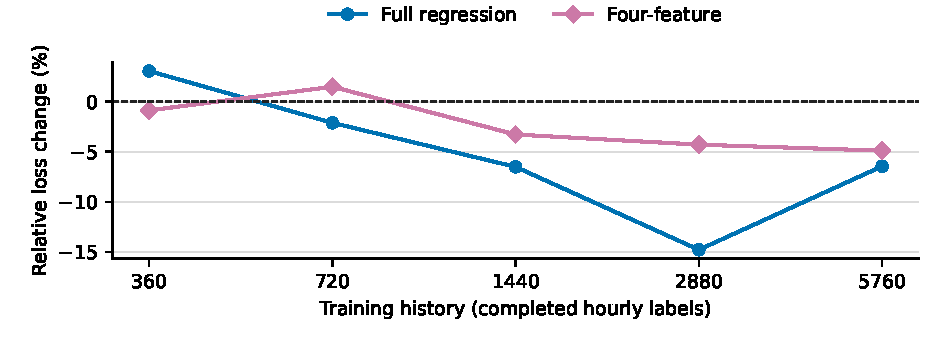
\includegraphics[width=.88\linewidth]{figures/v11-fx-history.pdf}
\caption{Saved short-horizon FX learning curves on the original evaluation period. The methods retain distinct original penalty menus, and every tested history is shown against its own matched historical headroom. This retrospective comparison does not identify a universally optimal history.}\label{fig:v11-history}
\end{figure}
\FloatBarrier

\paragraph{A fixed CFTC history-length extension}\label{par:wp2-history}
A fixed extension, committed locally before calculation and uploaded publicly afterward, examines the short-history pattern across 17 CFTC aggregate dealer-position markets. Its fixed horizon is six weeks. The 52- and 260-week results were already known and are reused unchanged; only the 520-week forecasts were new. Both prewritten low-history screens pass: QR4 loses to its matched rolling reference in 15 of 17 cells and QR33 in 29 of 34. The high-history QR4 screen fails, because 10 of 17 wins (58.8\%) fall below the fixed 60\% rule; strict improvement over all three windows holds in only 6 of 17 markets. Full regression has no prewritten high-region cell, leaving its high-history screen untestable. The primary verdict is therefore partial support. These dependent aggregate-market counts describe transport of a fixed prediction; they do not establish a generally sufficient financial history, a causal estimation-cost mechanism, or dealer-level replication. Supplement Section S39 gives all decision screens and counterexamples.

\subsection{RQ2: daily, weekly and independently reported positions}

The reference-sensitive hourly results motivate comparisons with other measurement clocks and reporting systems, each retaining matched histories and completed peak labels.

At weekly frequency, the Treasury-bill comparison favors historical headroom on both accuracy and breaches, extending the adverse ranking beyond the hourly examples. The earlier short-window version retains its separate adverse result because it uses a different history (Table~\ref{tab:weekly}).

Stronger regularization narrows weekly panel losses but leaves historical rules ahead, with conservative selection choosing the intercept-only report in 17 of 26 earlier cells (Table~\ref{tab:weekly}). Its largest relative loss increase occurs in the Treasury-bill short-history, 24-step comparison, despite conservative selection.

Neither simpler conditioning nor fixed combinations establish a uniform weekly improvement, reinforcing the need to retain the historical benchmark in each comparison. Supplement Sections S16--S18 retain their complete losses and failures, including the headroom-recursion results (Tables S14--S17).

Returning to the same FX record, historical headroom wins seven of eight daily comparisons; the exception uses four predictors, history 260 and horizon 6, reducing loss by 3.0\%. It records 37 breaches versus 30 for matched headroom. Daily aggregation therefore preserves the score--breach disagreement while changing the leading forecast in most comparisons (Supplement Section S25).

\begin{table}[htbp]\centering\small
\caption{Weekly evidence across the original main comparison, added panel and earlier-period comparisons. Counts refer to related tasks rather than independent dealers. Stronger regularization narrows losses while leaving substantial failures.}\label{tab:weekly}
\begin{tabular}{>{\raggedright\arraybackslash}p{4.3cm}>{\raggedright\arraybackslash}p{4.7cm}>{\raggedleft\arraybackslash}p{2.7cm}>{\raggedright\arraybackslash}p{2.5cm}}\toprule
Comparison set & Procedure & Loss change / median (\%) & Higher-loss cells\\\midrule
Original Treasury-bill main comparison & Original regression, long history & +50.79 & Original main comparison\\
Earlier Treasury-bill short-window version & Short-history short-window version & +144.30 & Different history\\
Additional panel & Original full regression & +92.63 & 45 / 48\\
Additional panel & Four-feature regression & +9.91 & 37 / 48\\
Additional panel & Full regression, expanded penalties & +9.22 & 34 / 48\\
Additional panel & Ordinary empirical headroom quantile & +0.50 & 30 / 48\\
Earlier weekly groups & Validation-minimum expanded rule & +4.15 & 26 groups\\
Earlier weekly groups & One-standard-error rule & +5.37 & 26 groups\\
\bottomrule\end{tabular}
\par\smallskip\begin{minipage}{.98\linewidth}\footnotesize The original bill main comparison has 54 versus 28 strict breaches among 277 issues. Earlier short-history bill results use a different history; the one-standard-error worst excess is +181.39\%, and all its prewritten success criteria remain unmet. Supplement Sections S11--S15 list all panel and selection results (Tables S9--S13).\end{minipage}
\end{table}

\subsubsection{CFTC: independent reporting-system evidence}

The independent reporting system gives a similar overall ranking: a historical headroom rule has lower loss in 29 of 34 contract/history comparisons. This meets the pre-specified 60\% threshold, using the better realized score of corrected and ordinary empirical historical reports rather than an executable selector. Corrected historical headroom remains the fixed matched reference, with the ordinary empirical version reported separately. Both full-regression medians exceed the pre-specified ten-percent tolerance, whereas four-feature regression moves closer to history with the longer window. These comparisons extend the benchmark pattern to a separate reporting system while retaining substantial contract-level variation (Table~\ref{tab:v10-cftc-contracts}; Figure~\ref{fig:v10-cftc}).

\begin{table}[t]\centering\scriptsize
\setlength{\tabcolsep}{2pt}
\caption{CFTC dealer-category futures: relative loss versus matched historical headroom (\%). All 17 selected literal contract codes are retained.}
\label{tab:v10-cftc-contracts}
\resizebox{\linewidth}{!}{%
\begin{tabular}{l*{10}{r@{.}l}}\toprule
Contract & \multicolumn{10}{c}{History 52} & \multicolumn{10}{c}{History 260} \\
\cmidrule(lr){2-11}\cmidrule(lr){12-21}
code & \multicolumn{2}{c}{\shortstack{Intercept\\only}} & \multicolumn{2}{c}{\shortstack{Four-\\feature}} & \multicolumn{2}{c}{\shortstack{Full\\regression}} & \multicolumn{2}{c}{\shortstack{Calibrated\\history}} & \multicolumn{2}{c}{\shortstack{Calibrated\\regression}} & \multicolumn{2}{c}{\shortstack{Intercept\\only}} & \multicolumn{2}{c}{\shortstack{Four-\\feature}} & \multicolumn{2}{c}{\shortstack{Full\\regression}} & \multicolumn{2}{c}{\shortstack{Calibrated\\history}} & \multicolumn{2}{c}{\shortstack{Calibrated\\regression}} \\ \midrule
044601 & 5 & 26 & 128 & 00 & 41 & 38 & 15 & 01 & 18 & 80 & 0 & 51 & 7 & 82 & 43 & 88 & 13 & 87 & 42 & 41 \\
043602 & 3 & 37 & 9 & 35 & 3 & 37 & 37 & 79 & 24 & 64 & 2 & 30 & 8 & 95 & 20 & 97 & -11 & 22 & -12 & 64 \\
042601 & 4 & 64 & 9 & 48 & 35 & 65 & 26 & 69 & 41 & 21 & -0 & 15 & 74 & 23 & 16 & 63 & 1 & 46 & 9 & 39 \\
045601 & -2 & 04 & 0 & 31 & -2 & 04 & 21 & 83 & 6 & 14 & 1 & 85 & 1 & 85 & 1 & 85 & 2 & 40 & 2 & 58 \\
020601 & 4 & 77 & 79 & 72 & 111 & 12 & 25 & 66 & -5 & 34 & 0 & 92 & 43 & 38 & 29 & 70 & -15 & 12 & -12 & 32 \\
099741 & 0 & 69 & 13 & 97 & 14 & 56 & 77 & 33 & -13 & 28 & 0 & 22 & 0 & 22 & 0 & 22 & 27 & 72 & 27 & 73 \\
1170E1 & 6 & 42 & 6 & 82 & 46 & 30 & -0 & 22 & 12 & 77 & 0 & 92 & -28 & 44 & -16 & 22 & -1 & 12 & 1 & 00 \\
097741 & -0 & 83 & 23 & 76 & 68 & 71 & 29 & 77 & 33 & 79 & 0 & 53 & -6 & 54 & 14 & 69 & -0 & 41 & -5 & 43 \\
096742 & 2 & 93 & 3 & 41 & 6 & 13 & 49 & 54 & 30 & 46 & 5 & 30 & 4 & 82 & 62 & 68 & 37 & 12 & -0 & 49 \\
095741 & 7 & 39 & 19 & 55 & 19 & 33 & 41 & 27 & 42 & 98 & -0 & 70 & 2 & 13 & 10 & 35 & 19 & 30 & 55 & 39 \\
090741 & 4 & 03 & 10 & 28 & 4 & 03 & 15 & 58 & 13 & 13 & 3 & 28 & -5 & 35 & -3 & 60 & -2 & 02 & -5 & 66 \\
232741 & 0 & 11 & 123 & 33 & 37 & 53 & 63 & 84 & 36 & 35 & 1 & 94 & -3 & 35 & 7 & 68 & -0 & 65 & -3 & 86 \\
33874A & 6 & 95 & 88 & 57 & 38 & 30 & 30 & 15 & 44 & 07 & -2 & 38 & -3 & 21 & -4 & 78 & 6 & 98 & 9 & 52 \\
240743 & -3 & 04 & -7 & 32 & 183 & 12 & 33 & 14 & 49 & 77 & -2 & 28 & -2 & 28 & -2 & 28 & 32 & 91 & 26 & 37 \\
092741 & 0 & 54 & 0 & 54 & 0 & 54 & -1 & 74 & -0 & 68 & 0 & 17 & -6 & 98 & 26 & 22 & 5 & 58 & 13 & 94 \\
098662 & -0 & 44 & -0 & 44 & 0 & 90 & 44 & 89 & 38 & 90 & 2 & 45 & -39 & 44 & 2 & 45 & 15 & 12 & 20 & 45 \\
112741 & 11 & 06 & 38 & 76 & 10 & 05 & 33 & 72 & 24 & 10 & 2 & 24 & 2 & 82 & 80 & 98 & 8 & 36 & 16 & 37 \\
\bottomrule\end{tabular}}
\par\vspace{2pt}\begin{minipage}{.98\linewidth}\footnotesize
Entries are percentage loss differences from matched corrected historical headroom; positive values mean higher loss, and unavailable entries retain failed or incomplete comparisons.
The pre-specified conditions require historical superiority in at least 60\% of all 34 comparisons, full-regression medians within ten percent at both histories, and a strictly smaller four-feature median with longer history.
Full-precision results determine the comparisons, with all scores, breaches, selections and failures retained in Supplement Section S30.
\end{minipage}\end{table}


\begin{figure}[htbp]\centering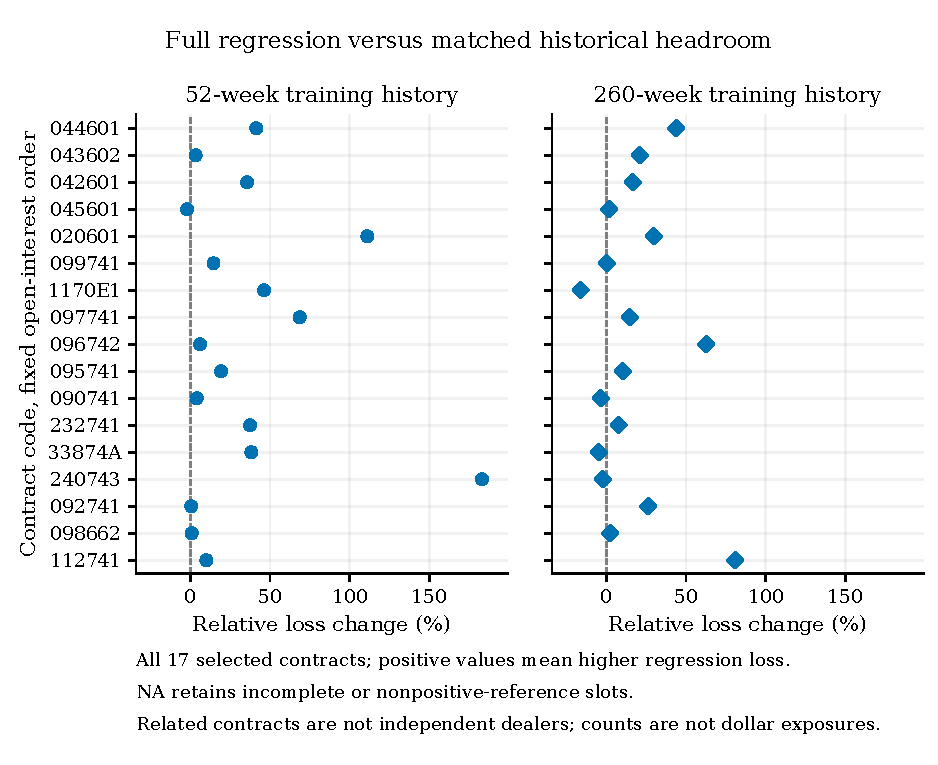
\includegraphics[width=.97\linewidth]{figures/v10-cftc-contract-changes.pdf}
\caption{Expanded-menu regression relative loss versus matched historical headroom for every eligible CFTC contract. Columns separate histories; code order follows the fixed open-interest ranking. Positive values mean higher regression loss.}\label{fig:v10-cftc}
\end{figure}

\subsubsection{Model confidence sets}

Matched historical methods remain in most confidence sets, usually alongside alternatives (Supplement Table~\vthirteenMCSTable{}). Non-elimination establishes neither equal predictive risk nor a uniquely preferred method, supporting the retention of historical controls as comparators.

% Display-only generated file; exact saved-number bindings are in notes/v12/new-paper-number-bindings.json.
\FloatBarrier
\subsection{Finite-menu loss decomposition and validation length}\label{sec:v12-low-frequency}
Loss from penalty selection exceeds half of positive actual excess loss in 27 of 41 short-history weekly comparisons (Figure~\ref{fig:v12-decomposition}). Extending validation lowers CFTC median excess loss from 19.33\% to 4.03\% with short histories, and from 10.35\% to 0.53\% with longer histories. The New York Fed medians fall from 6.68\% to -1.13\% at horizon six and from 40.47\% to 5.02\% at horizon twenty-four (Table~\ref{tab:v13-validation}). Yet the best finite penalty selected with evaluation hindsight still loses to historical headroom in 29 of 41 comparisons. This gap describes the tested finite procedures; it does not establish that conditional information is absent.

The decomposition separates the selected report's gap from the best finite candidate and that candidate's gap from historical headroom. The retrospective finite candidate uses five penalties and excludes the ordinary empirical limit, supplying a diagnostic rather than a deployable selection rule. Separate component medians need not add: actual excess is 19.44\%, selection 18.32\%, and the diagnostic gap 4.37\%. An empirical-limit selection can beat every finite candidate, making its selection component negative; both long-history FX horizons have negative finite-menu gaps.

\begin{figure}[htbp]\centering
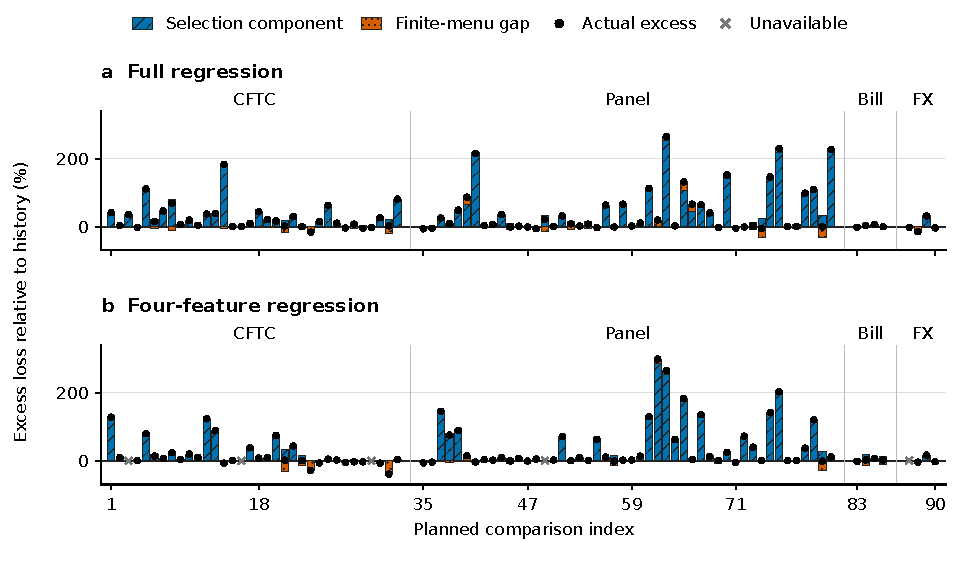
\includegraphics[width=.98\linewidth]{figures/v12-decomposition.pdf}
\caption{Signed decomposition of regression excess loss against matched historical headroom, with selection in blue, the finite-menu diagnostic gap in orange, and actual excess as black dots. Crosses retain unavailable comparisons; all planned comparisons remain plotted. Bill denotes Treasury bills; Panel denotes the twelve additional New York Fed series.}\label{fig:v12-decomposition}
\end{figure}

\begin{table}[htbp]\centering\small
\caption{Full-regression excess loss versus matched historical headroom under longer validation. Entries are source medians in percent; the final column counts selections of the intercept-only limit.}\label{tab:v13-validation}
\begin{tabular}{lrrrrrr}\toprule
Reporting system & Horizon & History & Series & Validation 52 & Validation 156 & Limit selections\\\midrule
CFTC & 6 & 52 & 17 & +19.33 & +4.03 & 4 to 10 \\
CFTC & 6 & 260 & 17 & +10.35 & +0.53 & 4 to 5 \\
New York Fed & 6 & 52 & 13 & +6.68 & -1.13 & 6 to 9 \\
New York Fed & 24 & 52 & 13 & +40.47 & +5.02 & 3 to 9 \\
\bottomrule\end{tabular}
\par\vspace{2pt}\begin{minipage}{.98\linewidth}\footnotesize
Lengths count weekly records; evaluation dates remain unchanged. New York Fed horizon six also moves the validation endpoint and refit phase; across-arm medians are not typical paired changes.
Supplement Section S38 gives individual series, four-feature results and the complete figure.
\end{minipage}\end{table}


Longer validation selects the intercept-only limit more often in both reporting systems, consistent with less aggressive conditional fitting (Table~\ref{tab:v13-validation}). The New York Fed horizon-six endpoint also advances eighteen weeks and changes the refit phase, leaving a causal length-only effect unidentified. Its median paired change is zero despite the lower long-validation arm median, so differences between arm medians need not represent typical improvements. The four-feature short-horizon New York Fed median-improvement screen fails. Its complete results and original CFTC failures remain available in Supplement Sections S36 and S38. The simulation menu comparison also brings short-history regression closer to history, linking these outcomes to the tested histories, validation windows and shrinkage menus.

\FloatBarrier

Tail-level sensitivity remains incomplete (Table~\ref{tab:v12-tau}). At 99\%, one CFTC failure leaves the 29-win criterion unresolved despite 28 historical wins in 34 comparisons. Required numerical fits fail in both FX periods, leaving joint improvement undetermined. After a solver repair designed after the failure, only 6 of 10 compatibility fits met the forecast-preservation criterion. The rejected repair leaves all three failed cells and original judgments unchanged.

\begin{table}[htbp]\centering\small
\caption{Full-regression relative excess loss (\%) at alternative quantile levels. Positive values favor matched historical headroom; NA retains any failed required comparison.}\label{tab:v12-tau}
\begin{tabular}{lrr}\toprule
Source / training history & 90\% & 99\% \\\midrule
CFTC, 52 weeks & +3.45 & +15.05 \\
CFTC, 260 weeks & +1.58 & \textsc{NA} \\
FX, original period & -10.15 & \textsc{NA} \\
FX, earlier period & -17.85 & \textsc{NA} \\
Treasury bills & +0.67 & +44.22 \\
\bottomrule\end{tabular}
\par\vspace{2pt}\begin{minipage}{.95\linewidth}\footnotesize
Contract rows give full-group medians; histories are 2,880 hours for FX and 260 weeks for Treasury.
The rejected post-failure repair leaves original NA entries unchanged (Supplement Section S38).
\end{minipage}\end{table}


\subsection{Scores and breach behavior answer different questions}

Lower pinball loss leaves breach behavior unresolved: matched FX gains accompany more breaches before calibration (Table~\ref{tab:fx}). Elementary-score curves cross in both original comparisons (Supplement Figures S2--S3); the separate 24-step comparison reverses near 20.6:1 (Section S9, Table S8). Both six-step FX comparisons reduce mean underprediction and overprediction, so that weight reversal belongs to the longer-horizon reference. Average-loss tests, strict-hit diagnostics and RMS-state comparisons therefore answer distinct questions (Supplement Table S47; \citealp{gw2006}).

\FloatBarrier

\section{RQ3: limit-cost regions}\label{sec:cost}

\[
J_m(\kappa,\beta,c)=\kappa\frac{\overline{C_m-B}}{m_F}
+\beta\,\overline{\mathbf 1\{Y>C_m\}}
+c\frac{\overline{(Y-C_m)_+}}{m_F},\qquad
m_F=\overline{C_F-B}>0,\quad\beta=b/m_F.
\]

For CFTC, higher reserve coefficients and lower fixed-breach coefficients generally favor expanded-menu regression over matched historical headroom, although the grid is not monotone (Figure~\ref{fig:v10-cost}).
At $c=1$, regression is strictly cheaper in $5/34$ comparisons at the center of the sorted grid $(\kappa,\beta)=(.1,.25)$, $32/34$ at $(1,0)$, and $1/34$ at the opposite corner $(.01,5)$.
These are illustrative costs, not observed operating costs; Supplement Section S32 gives the normalization, fixed grid and complete-method results.

\begin{figure}[p]\centering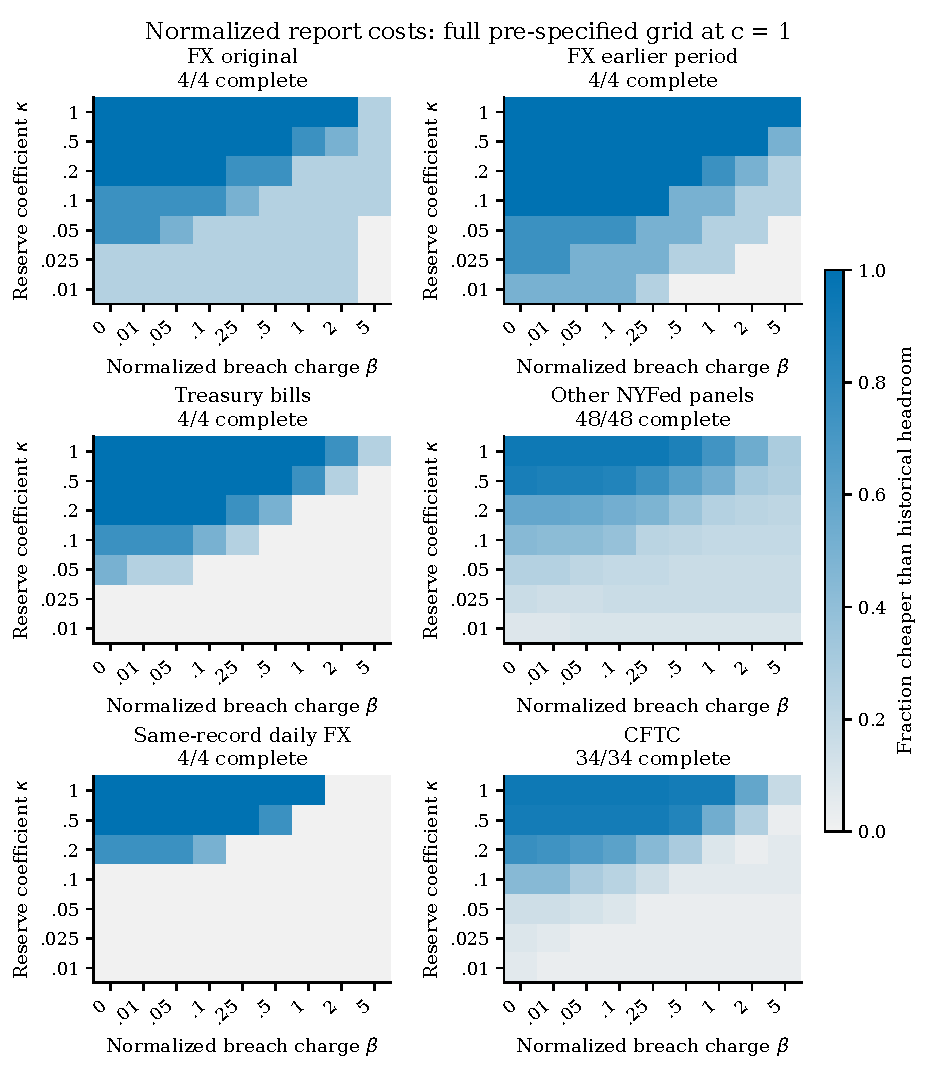
\includegraphics[width=.98\linewidth,height=.87\textheight,keepaspectratio]{figures/v10-cost-regions.pdf}
\caption{Fixed reserve and breach-charge regions with the exceedance coefficient held at unity. Color shows the fraction of related comparisons where the stated conditional procedure costs less than corrected historical headroom, with each source group retaining its own histories and horizons. These are descriptive fractions; all comparisons are complete, and the lower and upper fractions coincide.}\label{fig:v10-cost}
\end{figure}

\FloatBarrier

\section{Implications for model validation}\label{sec:implications}

\subsection{A benchmark-default validation protocol}\label{sec:v13-rp}
The protocol combines the six-point menu in Table~\ref{tab:methods}, longer validation and a corrected-rank historical default. It selects the lowest mean validation loss over 156 weekly observations or 5,760 FX records. The selected candidate replaces historical headroom only when its paired validation improvement strictly exceeds one HAC standard error \citep{nw1987}. Across 60 weekly comparisons, the protocol retains historical headroom in 32 and has 0.00\% median excess, compared with 14.63\% for ordinary regression. This zero median reflects the majority of decisions retaining historical headroom. However, 8 cases lose by over ten percent, exceeding the prewritten five-percent ceiling for such cases; the worst excess is 80.98\% (Figure~\ref{fig:v13-rp}). Both FX periods retain the ordinary regression gains, meeting the criterion for retaining gains. The rule was designed after earlier findings and uses inspected evaluation periods, so this check is retrospective.

\begin{figure}[htbp]\centering
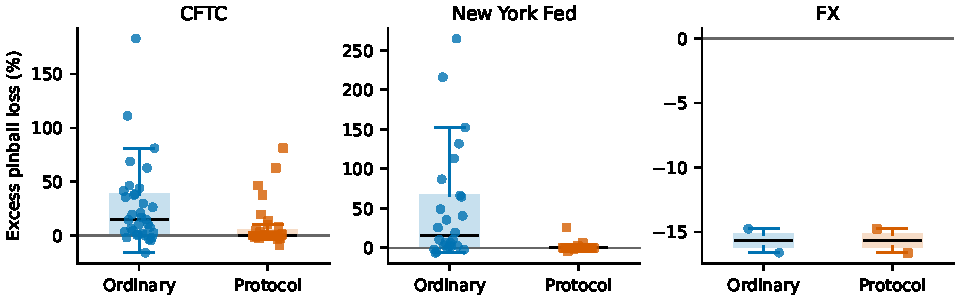
\includegraphics[width=.98\linewidth]{figures/v13-rp.pdf}
\caption{Ordinary regression and the benchmark-default protocol relative to matched historical headroom. Every planned comparison is complete: 34 CFTC, 26 New York Fed and two FX cases; points retain each outcome, including large losses. Separate vertical scales preserve each source's distribution without pooling native exposure units.}\label{fig:v13-rp}
\end{figure}

\subsection{Practical reporting}


\textbf{Benchmark against historical headroom.} Use the same completed labels, history length and refit schedule, naming the shorter rolling reference separately because its FX ranking changes across periods. This keeps differences in available history distinct from the gains associated with conditioning within a matched comparison.

\textbf{Use historical headroom by default when validation evidence is short.} Longer validation and a paired standard-error gate improve the weekly median, but leave eight large losses in the complete comparison (Section~\ref{sec:v13-rp}). Passing this gate alone therefore fails to establish adequate benchmark protection. The ordinary empirical quantile is up to 36.5\% worse than corrected headroom in the earlier weekly grid, supporting a separately validated historical default.

\textbf{Report breaches with the score.} Show mean underprediction, mean overprediction and strict-breach counts together, since the unwrapped matched FX gain and daily regression exception both accompany more breaches than history. Cost regions add reserve, breach-frequency and exceedance preferences to this joint evaluation.

\FloatBarrier

\section{Limitations}\label{sec:limitations}

\begin{itemize}\setlength{\itemsep}{0pt}\setlength{\parskip}{0pt}
\item FX comes from one market maker, and its original evaluation period was inspected before conditional methods were specified.
\item The earlier-period comparison and full-prefix backcast are retrospective, with no previously unseen prospective financial evaluation.
\item Weekly reports aggregate positions across dealers; related categories and the CFTC survivor universe do not provide independent dealer replications. Net-position peaks summarize exposure; gross portfolios, hedging arrangements and economic capital requirements remain unidentified.
\item Downloaded economic-date vintages omit historical first-release information, reporting delays and unrecorded within-interval excursions.
\item The comparisons identify neither causal effects nor individual-feature effects, and fitted limits receive no coverage guarantee under this dependence.
\item Costs illustrate fixed preferences; trading returns, funding gains and institutional intervention costs are not measured.
\item The finite-penalty hindsight bound is diagnostic only; validation-length and quantile-sensitivity checks are post-result analyses with numerical failures retained.
\item Only 6 of 10 high-quantile compatibility fits pass, so the rejected repair leaves both FX comparisons unavailable.
\end{itemize}
Supplement Section S36 retains the original technical qualifications on simulations, aggregation and forecast comparison. A consolidated register in Supplement Section S40 retains supported, unsupported and untestable prewritten screens.

\FloatBarrier

\section{Conclusion}\label{sec:conclusion}

Historical rules are hard to beat. For RQ1, matched FX regression gains recur across periods, but a shorter rolling reference changes the ranking (Table~\ref{tab:fx}). The learning curve also gives back part of its gain at the longest history, linking conditional performance to available history rather than universal model advantage (Figure~\ref{fig:v11-history}).

For RQ2, longer validation reduces full regression medians in both weekly reporting systems, but across-arm differences need not describe typical paired improvements (Table~\ref{tab:v13-validation}). These dealer aggregates remain related tasks, and the horizon-six New York Fed extension also moves the validation endpoint. The benchmark-default protocol cuts weekly median excess to 0.00\% and preserves FX gains, yet 8 of 60 cases still lose by over ten percent, with a worst excess of 80.98\% (Section~\ref{sec:v13-rp}). This failed tail criterion limits the protocol's risk-management recommendation, and the rejected high-quantile repair leaves its original judgments unresolved.

For RQ3, higher reserve charges and lower fixed breach charges generally favor expanded regression in CFTC, with local exceptions (Figure~\ref{fig:v10-cost}). Lower pinball scores can therefore coexist with more breaches and different cost rankings, requiring joint reporting of reserve amounts, breach counts and exceedance amounts. The costs are stipulated preferences rather than observed institutional costs, and the financial evidence remains retrospective.

\FloatBarrier

\section*{Data and code availability}
\paragraph{Data availability} The FX input is the specified version of the Kaggle Net Position Time Series Dataset. The owning metadata labels its license ``Data files \copyright\ Original Authors.'' This repository supplies the acquisition route and input fingerprint, but excludes raw FX observations and private per-issue prediction vectors. Obtain the source from \url{https://www.kaggle.com/datasets/davidlindsay1979/net-position-time-series-dataset} subject to the original rights holders' terms.

The New York Fed aggregates are available from its Primary Dealer Statistics service under the Bank's Terms of Use. The repository preserves the unchanged accepted Treasury snapshot with attribution and identifies study calculations separately. Copying or distributing that content remains subject to its source notices, attribution, modification labeling, continuing conditions and endorsement restrictions: \url{https://www.newyorkfed.org/privacy/termsofuse.html}. Software availability does not replace those source conditions. The original panel CSV is not redistributed, and current public vintages need not reproduce its exact input bytes.

The CFTC application uses the public Traders in Financial Futures (TFF) historical files from \url{https://www.cftc.gov/MarketReports/CommitmentsofTraders/HistoricalCompressed/index.htm}. The repository includes unchanged downloaded records and a per-file URL, acquisition time, byte count and SHA-256 record in \texttt{data/cftc-tff/provenance.json}.

\paragraph{Code availability} Code, written protocols, aggregate results and reproduction instructions are available in the \href{https://github.com/ByronLi0207/financial-mathematics-paper-20261020/tree/submission-final}{versioned repository}. Full financial replay also requires the documented original inputs and historical Git objects. [AUTHOR TO ADD ZENODO DOI AND CONFIRM SOFTWARE LICENSE].

\section*{Author-provided information}
Author information: [TO BE COMPLETED BY AUTHOR].\par
ORCID: [TO BE COMPLETED BY AUTHOR].\par
Funding: [TO BE COMPLETED BY AUTHOR].\par
Competing interests: [TO BE COMPLETED BY AUTHOR].\par
CRediT contributions: [TO BE COMPLETED BY AUTHOR].\par
Permissions and data-sharing exception: [TO BE CONFIRMED BY AUTHOR].\par

\bibliographystyle{rQUF}
\bibliography{references}
\end{document}
